\documentclass[oneside,openright,frontopenright]{dmathesis}
\usepackage[utf8]{inputenc}
\usepackage[T1]{fontenc}
\usepackage{lmodern}
\usepackage[british]{babel}
\usepackage[figuresright]{rotating}
\usepackage[draft=false,protrusion=true,expansion,shrink=10,stretch=10,]{microtype}
\makeatletter
\@ifpackageloaded{microtype}{%
	\providecommand{\disableprotrusion}{\microtypesetup{protrusion=false}}
	\providecommand{\enableprotrusion}{\microtypesetup{protrusion=true}}
}{%
	\providecommand{\disableprotrusion}{}
	\providecommand{\enableprotrusion}{}
}
\makeatother

\usepackage{csquotes}


\usepackage{amsmath,amsthm,amssymb}
\usepackage[hidelinks,draft=false]{hyperref}
\usepackage{booktabs}
\usepackage{xfrac}

% The folder in which images are stored for this project.
% If this is enabled, the folder doesn't need to be specified in each
% call to \includegraphics, i.e
%   \includegraphics{picturename}
% rather than
%   \includegraphics{img/picturename}
%\graphicspath{./img}

% Thmtools sets up theorem-like environments, and modifies the autoref
% command from hyperref to work when these environments share a counter
% Thmtools also defines an Autoref command for capitalising at the start
% of a sentence
\usepackage{thmtools}
\declaretheorem[
style=plain,
name=Theorem,
numberwithin=section
]{thm}
\declaretheorem[
style=plain,
name=Proposition,
numberlike=thm
]{prop}
\declaretheorem[
style=plain,
name=Lemma,
numberlike=thm
]{lem}
\declaretheorem[
style=plain,
name=Corollary,
numberlike=thm
]{cor}
\declaretheorem[
style=definition,
name=Definition,
numberlike=thm
]{mdef}
\declaretheorem[
style=definition,
name=Example,
numberlike=thm
]{example}
\declaretheorem[
style=definition,
name=Remark,
numberlike=thm
]{rem}
\declaretheorem[
style=plain,
name=Conjecture,
numberlike=thm
]{conj}
\declaretheorem[
style=plain,
name=Question,
numberlike=thm
]{question}

\numberwithin{equation}{section}
\allowdisplaybreaks

% Makes the last line of a page flush wtih the bottom margin for neatness
%\raggedbottom
%\emergencystretch=1em
\flushbottom

% use these to make paragraphs not indented,
% and to separate consecutive paragraphs
\setlength{\parindent}{0pt}
\setlength{\parskip}{0.5em plus 3pt minus 3pt}

% Provide itemize without extra spacing
\newenvironment{itemize*}%
{\begin{itemize}%
	\setlength{\itemsep}{0pt}%
	\setlength{\parskip}{0pt}}%
{\end{itemize}}
\newenvironment{enumerate*}%
{\begin{enumerate}%
	\setlength{\itemsep}{0pt}%
	\setlength{\parskip}{0pt}}%
{\end{enumerate}}

% Format captions
\usepackage[margin=15mm,hang]{caption}
\usepackage{subcaption}

\setfloatlocations{figure}{tbp}
\setfloatlocations{table}{tbp}

% In align*, use this to number a particular line
% Rather than using align, and \nonumber-ing every other line
\newcommand\numberthis{\addtocounter{equation}{1}\tag{\theequation}}
% Change autoref names. Generally I want sections to be capitalised at all
% times, not just when starting a sentence.
% (I'm not sure whether all these are necessary nor what the defaults are)
\renewcommand{\equationautorefname}{equation}
\newcommand{\equationAutorefname}{Equation}
\newcommand{\sectionAutorefname}{Section}
\newcommand{\chapterAutorefname}{Chapter}
\newcommand{\subsectionAutorefname}{Subsection}
\newcommand{\subsubsectionAutorefname}{Subsection}
\newcommand{\algorithmAutorefname}{Algorithm}
% Annoyingly these defs need to come *after* \begin{document}, so add to begin
% document hook.
\AtBeginDocument{%
	\def\sectionautorefname{Section}%
	\def\chapterautorefname{Chapter}%
	\def\subsectionautorefname{Subsection}%
	\def\subsubsectionautorefname{Subsection}%
	\def\algorithmautorefname{Algorithm}%
}
\usepackage{cite}
\begin{document}
\title{Null geodesics}
\subtitle{Modelling light in the Schwartzschild metric}
\author{Joseph A Sweeney}
\researchgroup{Mathematics}
\pagenumbering{roman}
\maketitlepage*

\begin{abstract}
%
	In this paper I will show and discuss my findings on numerical methods and optimisations for modelling solutions to the equations of motion deried from geodesic equations in the Schwarzschild and Kerr metric using Python. In the first section, I will introduce some key information and language associated with General Relativity, which this paper will rely upon. Then, I will demonstrate methods for modelling null (light-like) geodesics about a metric. Using these I will model various black holes as seen directly in front of an observer with any given celestial sphere.
%
\end{abstract}

\begin{declaration*}
%
	The work in this thesis is based on research carried out in the Department of
	Mathematical Sciences at Durham University. No part of this thesis has been
	submitted elsewhere for any degree or qualification.
%
\end{declaration*}

\disableprotrusion
\tableofcontents*
\enableprotrusion

\cleardoublepage
\pagenumbering{arabic}

%\include{background}
%\include{paper1}
%\include{paper2}
%\include{paper3}
\begin{introduction}

	The field of black hole imaging in Physics and Computer Science had a wave of enthusiasm 
	and development following Christopher Nolan’s 2014 blockbuster Interstellar\cite{Interstellar}, and the imaging of the supermassive 
	black hole at the centre of M87 by the Event Horizon Telescope in 2019\cite{event2019first}. Producing high quality images 
	and videos of black holes and wormholes can be very computationally costly, so ingenious ways of gaining 
	efficacy must often be used. My aim is to explore these methods and tricks to present practical approaches 
	to modelling the Schwarzschild metric and Kerr metric. After this I will explore accretion discs and gravitational redshift to create as realistic a model as possible.

\end{introduction}

\chapter{Introduction to General Relativity}
	Albert Einstein’s theory of General Relativity is a pivotal achievement in the scientific community, here, I will attempt to briefly summarise some key components and notation for ease of readers in later sections.

	In his theory of General Relativity, Einstein formalised gravity not as a force - as it is thought of in Newtonian physics - but as the curvature of spacetime. Spacetime is the 4-dimentional plane we exist in, one dimension representing time, and three space. The path of an object acted upon solely by gravity can be thought of as moving along curved spacetime, with the path being a straight line if the effects of gravity are non-existent. Such a path through curved spacetime is called a geodesic, and equations of motion in General Relativity are governed by constants derived from geodesic equations – which in turn are derived from the metric in which the object finds itself. A null-geodesic, or light-like geodesic, is a path describing the motion of a massless object: In this paper, a null-geodesic will always be describing the path of a light particle in a metric. Geodesic equations can be thought of as a generalisation of Newton's second law of motion, taking into account the curvature of the spacetime one chooses. I.e instead of F = 0 $\Rightarrow$ a = 0, we have that F = 0 implies that acceleration is sufficient to keep the motion in a straight line when considered in ordinary space.

	As is common in papers studying light and the astrological, I will be using natural units: That is, I will be taking c = G = 1, this results in non-SI units, but conversion is possible and generally simple. A distance of 1 will correspond to $1$(s) x c($ms^{-1}$) = the distance travelled by light in a vaccum in one second.

	The celestial sphere from a point in space is an image of all the points taken to be arbitrarily far away - for earth it is the sky in all directions excluding the moon, mercury and mars. (My 'arbitrary distance' is t=1000 i.e the distance light travels in a vaccum in 1000 seconds)

	Metrics are sections of spacetime which are solutions to Einstein’s field equations, the equations that define his General theory. As an example, the simplest solution to these field equations describing a black hole is the Schwarzschild metric. A metric is generally given in line notation - which informs one how a change in space relates to changes in the variables we consider the object to be moving in. The relation between geodesic equations and metrics are governed by Christoffel symbols, denoted $\Gamma$, seen in the below general form of a geodesic equation\cite{geodesic}:  


	\[\frac{d^2 \gamma^\lambda}{dt^2} + {\Gamma^\lambda}_{\mu\nu} \frac{d\gamma^\mu}{dt} \frac{d\gamma^\nu}{dt} = 0\]

	Christoffel symbols are incredibly important in the study of General Relativity, relating directly to the Riemann tensor, Metric tensor and other key concepts. Below I will give a sense as to what they represent, but will not dive any further, standing on the shoulders of giants by relying on equations derived and examined over many years.

	The Christoffel symbols are related to the coefficients in the line metric, and can be quite messy as they consider all relations between variables. Below is the general form of the Christoffel symbol using Einsteins summation convention\cite{albert1916foundation}:
	
	\[{\Gamma^\lambda}_{\mu\nu} = \frac{1}{2}g^{\lambda{l}}(\partial_{\nu}g_{\mu{l}} + \partial_{\mu}g_{l\nu} + \partial_{l}g_{\mu\nu})\]
	
	Here, g is the matrix of coefficients in the metric - g is also confusingly called the metric but this is as it determines the line notation completely. $g_{ij}$ is the (i,j)'th component of g, and $g^{ij} = {g^{-1}}_{ij}$ is the (i,j)th component of the inverse of g.

\chapter{Solving general relativistic equations of motion}

	Equipped with the equations of motion derived from the geodesic equation determined by the metric we are given; we can visualise the path of light in such a metric by solving these equations numerically.


\section{Deriving the equations of motion}
	
	We will start with the Schwarzschild metric, given in line notation by\cite{derivationSchwarzschild}: 


	\[{ds^{2} = {\left(1-\frac {2m}{r}\right)}^{-1}} {dr^2} + {r^2}({d\theta ^2} + {\mbox{Sin} ^2}{\theta}{d\varphi ^2}) -{\left(1-\frac {2m}{r}\right)}{dt^2}\]


	Since the metric is spherically symmetric, we see that every path will always be contained in a plane intersecting the origin of the black hole. Therefore, without loss of generality we can take ${\theta}=\frac{\pi}{2}$ and observe from 'above’ the equatorial plane to see the path of such a light ray in the plane.

	Observing that the Schwarzschild metric is time independant implies that the energy of a photon in the metric will be constant (equal to its value at t=0). Similarly, independance from the variable $\varphi$ leads us to see that the $\varphi$ component of the angular momentum of a photon in the Schwarszchild metric remains constant. We call these contants E (= -$p_0$) and L (= $p_\varphi$) respectively. Since we take ${\theta}$ to be constant, $p_\theta$ = 0 as the angular momentum in the $\theta$ plane is proportional to $\frac{d\theta}{dt} = 0$.

	For the other components of the photons momentum:

	\[p^0 = g_{00}p_0 = \frac{rE}{r-2M} \]
	\[p^r = \dot{r}\]
	\[p^\varphi = g^{\varphi\varphi}p_\varphi = \dot{\varphi} = \frac{L}{r^2}\]

	Using the equation $p \cdot p$ = 0 we see that:

	\[-\frac{rE^2}{r-2m}+\frac{r\dot{r}^2}{r-2M}+\frac{L^2}{r^2}=0\]

	This equation can be solved, leading to the equation:

	\[\dot{r}^2 = E^2-\frac{L^2(r-2M)}{r^3} = E^2 + V^2\]

	Here we let let V = V(r) for ease of notation.

	Then, taking the time derivative of both sides of this equation:

	\[2\dot{r}\ddot{r} = -\frac{d}{dr}(V^2)\dot{r}\]

	Calculating $\frac{d}{dr}(V^2)$ shows that the equations of motion of a photon in the Schwarzschild metric are governed by:

	\[\ddot{r} = -\frac{1}{2}\frac{d}{dr}(V^2) = -\frac{L^2(3M-r)}{r^4}\]
	\[\dot{\varphi}=\frac{L}{r^2}\]


	Where M is the mass of the black hole, L is a constant equal to the angular momentum of the light ray, r is the distance from the centre of the black hole, and $\varphi$ is the angle from the positive x axis to the light ray.

	In this section, usually instead of the time variable t, a more general variable such as $\lambda$ is used, but as we are not interested in modelling realistic animations, taking t as our variable does not affect the end result. The derivations in this subchapter were based on \cite{schutz2009first}.

\section{Method for solving the system}
	The simplest method of solving such an equation numerically is to split the equation into a coupled first order differential equation. Then use a numerical approximation to update r, $\dot{r}$ and $\varphi$ for each point in a time array, if you keep track of r and $\varphi$ for all points in the time array you can then plot the path. One thing to be careful about is that as soon as light is within r = 2M, solutions will not make any sense, so we cannot have an initial position in this region, and ideally while keeping track of r, cut the process off when r = 2M.

	This method is both the simplest and most effective for solving second order ODE’s numerically, the only difference between a ‘bad’ and ‘good’ method would be the choice of numerical approximation method to solve the first order ODE’s.

	Below are the coupled differential equations equivalent to the equations of motion:

	\[\dot{r}= s\]
	\[\dot{s}=-\frac{L^2(3M-r)}{r^4}\]
	\[\dot{\varphi}=\frac{L}{r^2}\]

	I have found that for a plot of the path of a photon (See Figure 3.1), the ideal method is solve\_ivp\cite{2020SciPy-NMeth}, using LSODA\cite{hindmarsh2005lsoda}, this is as the Explicit Runge-Kutta method of order 5 (RK45)\cite{fehlberg1969low}, the inherent method used by solve\_ivp is very efficient but not smooth, so makes for unattractive plots. Later, when a plot is not required, I will be using RK45. Also, solve\_ivp allows one to keep track of an ‘event’, and return if the event took place, moreover one may choose to cut off the calculation process when such an event takes place. Naturally this is very useful in our case, as all we need to set the event to is r < 2M.


\chapter{Imaging a Schwarzschild black hole}

	We now have the means to start thinking about how to model a black hole of distance r away from a camera, with any given celestial sphere.

\section{Outline of the method}

	Firstly, we would like to find an equation linking launch angle and L, as this would allow us to choose a launch angle and calculate the required parameters for such an angle.

	Then, to model a Schwarzschild black hole we will first find the minimum angle one may fire a photon from the camera without the photon being absorbed by the singularity. For all angles between this minimum angle and just under $\frac{\pi}{2}$ (for this value I take 1.55), we will find a relation between angle fired and final angle after t=1000. The reason we do not go up to $\frac{\pi}{2}$ itself is because as seen later we take tan(launch angle), which of course is undefined at launch angle = $\frac{\pi}{2}$. L and the launch angle are directly correlated, so by taking L to be very large, we can see where the reasonable limit for us to calculate lies - this happens to be approximately 1.55.

	We will then conceptualise a pinhole camera, with its focal point, distance r from the centre of the black hole, the position of our camera which fires light rays. Using the relation outlined above, we can take any given line straight of pixels which passes through the centre of the image we take as our celesial sphere, and see where each pixel should end up. Then, by 'rotating' the pinhole camera - or by rotating this central line, we may find where each pixel in our new picture draws its light from on the celestial sphere.

\section{How to aquire the launch angle}

	For the rest of this paper we refer to a given photon's launch angle by $\alpha$. We would like to use the equations of motion at t = 0 to discover what value of L with given $\dot{r}$(0) leads to a specific $\alpha$.

	As we are in polar coordinates, 

			\[(x, y) = (r\mbox{Cos}(\varphi), r\mbox{Sin}(\phi)) \Rightarrow (\dot{x}, \dot{y}) = (\dot{r}\mbox{Cos}(\varphi) - r\dot{\varphi}\mbox{Sin}(\varphi), \dot{r}\mbox{Sin}(\varphi) + r\dot{\varphi}\mbox{Cos}(\varphi))\]
	
	Via basic geometry we see:
			
			\[\mbox{Tan}(\alpha) = \frac{\dot{y}(0)}{\dot{x}(0)} = \frac{\dot{r}(0)\mbox{Sin}(\varphi(0)) + r(0)\dot{\varphi}(0)\mbox{Cos}(\varphi(0)}{\dot{r}(0)\mbox{cos}(\varphi(0)) - r(0)\dot{\varphi}(0)\mbox{Sin}(\varphi(0))}\]

	So we obtain:

			\[ L = \frac{r(0)\dot{r}(0)(\mbox{Cos}(\varphi(0))\mbox{Tan}(\alpha)-\mbox{Sin}(\varphi(0))}{\mbox{Cos}(\varphi(0))+\mbox{Sin}(\varphi(0))\mbox{Tan}(\alpha)}\]

\section{Finding $\alpha_{min}$}
	
	To find the minimum angle at which a light ray escapes the gravitational pull of the black hole, I send out a number of photons with launch angles ranging from 0 to 1.55, then, as soon as an angle does not lead to a termination of solve\_ivp, I repeat this process with much smaller intervals between the previous and current angle. This leads to an accurate $\alpha_{min}$.

\section{The relationship between $\alpha$ and $\alpha^{'}$}

	By running this program across angles from $\alpha_{min}$ to 1.55 and plotting $\alpha$ on the x-axis with $\alpha^{'}$ on the y axis we find the relationship between $\alpha$ and $\alpha^{'}$. For $\alpha$ between -1.55 and -$\alpha_{min}$ we may take -f(-$\alpha$), where f is the function relating the two. Here we have covered -1.55 to 1.55 radii, more than a full field of view.

	Where  $\alpha^{'}$ is the angle from the camera to the final position of the light ray (See Figure 3.1).

	When $\alpha \approx \alpha_{min}$ or $-\alpha \approx -\alpha_{min}$ the light ray might semi-orbit or even fully orbit the black hole, meaning I had to be careful in my method  of calculating $\alpha^{'}$. To avoid errors I kept track of the change in $\varphi$, the angle from the current position of the ray to the centre of the black hole. When taking this value modulo $2\pi$, I could see how many orbits the ray had undergone. The main issue with not doing this is for a plot of the function (See Figure 3.2), in application we want the angle $-\pi<\alpha^{'}<\pi$.

\begin{figure}
	\centering
	\begin{minipage}{0.5\textwidth}
		\centering
		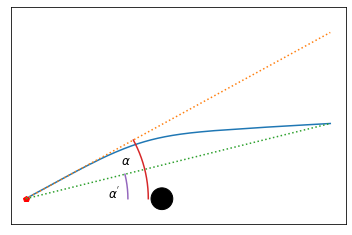
\includegraphics[width=0.8\linewidth]{img/alpha_alpha-prime}
		\caption{A plot with $\alpha$ = 0.5, $\alpha^{'}$ = 0.242 (t = [0,200], r(0) = 100, $\dot{r}$(0) = -1, $\varphi$(0) = -$\pi$, M = 4)}
	\end{minipage}%
	\hfill
	\begin{minipage}{0.5\textwidth}
		\centering
		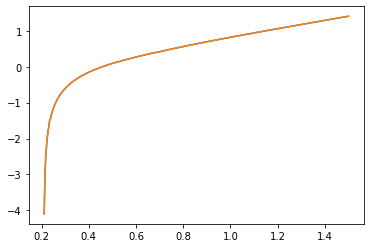
\includegraphics[width=0.8\linewidth]{img/alpha-prime_f(alpha)}
		\caption{A plot of the function f, relating $\alpha$ to $\alpha^{'}$ (t = [0,1000], r(0) = 100, $\dot{r}$(0) = -1, $\varphi$(0) = -$\pi$, M = 4)}
	\end{minipage}
\end{figure}

\section{Modelling the black hole}
	
	As outlined in 3.1, here we will give our code a star field to treat as a celestial sphere, and see how a black hole affects the image. To do this, the first thing we do is to calculate the distance in pixels from the middle of the picture to a corner, this will correlate directly to our 1.55 radians. Then, for every pixel on the original image we calculate the angle $\alpha$ implied by the distance from the pixel to the centre of the image. Then, we use numerical interpolation on our relationship between $\alpha$ and $\alpha^{'}$ to calculate the angle along the straight line intersecting the current pixel and the pixel at which the light ray would end. Then by converting this angle back to distance we update a copy of the picture to switch the current pixel for the closest pixel to the end point on the original picture.

\begin{figure}
	\centering
	\begin{minipage}{0.5\textwidth}
		\centering
		\includegraphics[width=0.8\linewidth]{img/8kstarfield-special}
		\caption{A model highlighting areas affected by the limited size of the image}
	\end{minipage}%
	\begin{minipage}{0.5\textwidth}
		\centering
		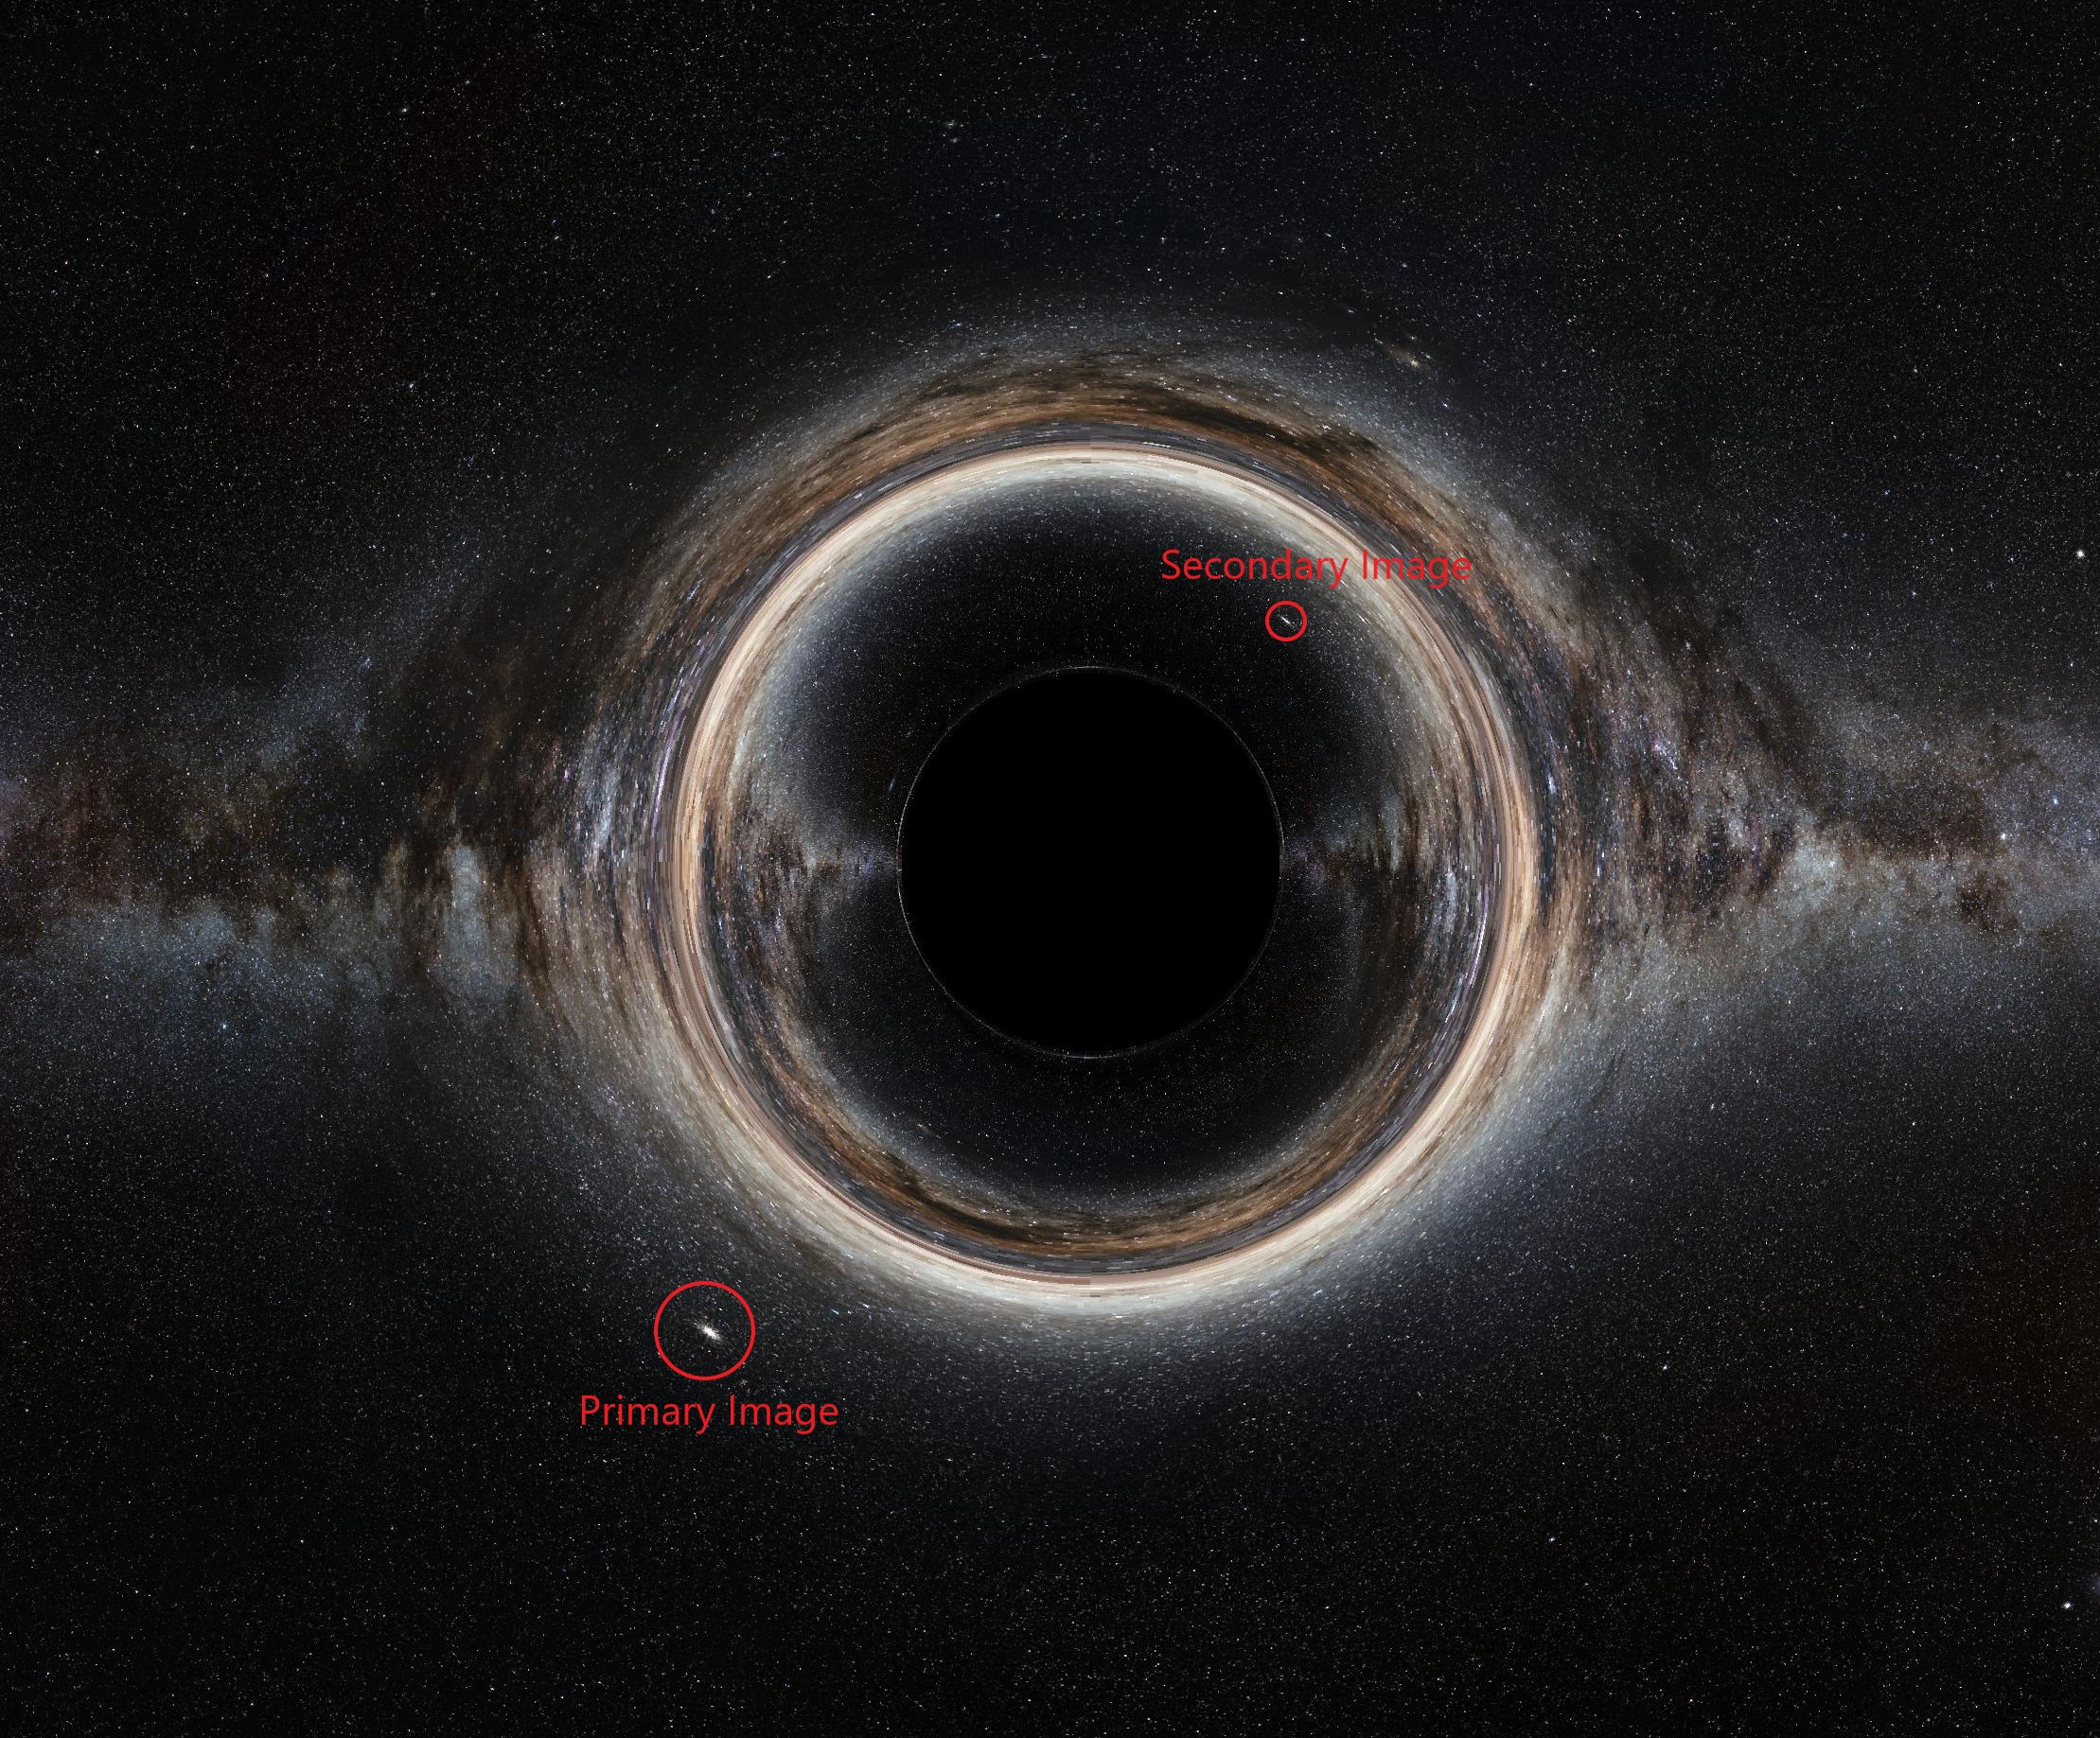
\includegraphics[width=0.8\linewidth]{img/hdri-pov}
		\caption{A model using a HDRI image, cropped to show POV. Credit for original image: Double Negative}
	\end{minipage}
\end{figure}

\section{The importance of a proper celestial sphere}

	One issue that I had when first modelling these black holes is that I was not using an image covering $4\pi$ steradians (2d equivalent of radians, $4\pi$ being a full field of view), meaning any ray which leaves the area covered by the original image would lead to a black pixel. This leads to an irregularly shaped black hole (See Figure 3.3), if the image I used as a celestial sphere was circular, the black hole would seemingly look ordinary, as the irregularities would be smoothed out horizontally and vertically, but would be too large. 

	My solution to this was to use a HDRI image, which indeed covers $4\pi$ steradians, and keeping models in this form - this is commonly done, notably in \cite{james2015gravitational}. It is simple to convert a HDRI image back to an ordinary POV image, but you are then limited to a small section of the information which can be seen in the original HDRI image. For example if one wanted to create an animation of a camera spinning in place in frozen time, one could rely solely upon one of these HDRI images.

	This does however change our previous method slightly, as HDRI images are designed to have the coordinates $\theta$ and $\varphi$, covering $2\pi$ and $\pi$ respectively, so instead of the distance to the corner of our image, we take the half the height of our image to be our $1.55$ radians. We are then limited to a maximum angle of 1.55 radians, meaning we may update the image only in a circle centred at the middle of the image, with radius $\frac{\mbox{height}}{2}$. Figure 3.4 is a cropped image of inside this circle.

	To be able to model light rays with angles equal to and above $\frac{\pi}{2}$, and hence to be able to take advantage of a full updated HDRI image, one must switch to the more general method of modelling black holes - relativistic ray tracing. As the purpose of this paper is to explore and explain effecient solutions I will not cover modelling a Schwarzschild black hole via relativistic ray tracing, however, in chapter 4 I will be using this method to model light in the Kerr metric.


\chapter{Kerr black holes}

	In this section I will move on to more general black holes, specifically ones with non-zero spin, I will introduce the Kerr metric and take a look at the equations of motions derived from the geodesic equation of light in the Kerr metric.

\section{Properties of black holes}

	Black holes are simultaniously one of the simplest and most complicated objects known to exist in the universe: On the one hand, we can only theorise what happens as black holes age, or what happens beyond the event horizon - but on the other, black holes are defined entriely by only three properties. This is extraordinary, especially when considering their size and significance.

	The three properties which define a black hole are mass, spin, and charge. Any two black holes with all three properties the same are essentially equivalent. Different metrics are given for describing black holes, these are usually to simplify things taking either spin or charge to be zero. For example the Schwarzschild metric, which we have been working with, is the simplest such metric - taking both spin and charge to be zero. The Kerr metric takes only charge to be zero, and spin affects the curvature of spacetime rather substantially. A charged, non-spinning black hole is described by the Reissner–Nordström metric, and finally, the most general metric describing a black hole is the Kerr-Newman metric - taking mass, spin and charge to all be non-zero. Of course one could use the equations of motion implied by the hamiltonian of the geodesic equation generated by the Kerr-Newman metric and take spin and/or charge to be zero rather than using other metrics - but this requires much more work.

\section{The Kerr metric}

	The Kerr metric of a mass M rotating with angular momentum a is given by \cite{raquepas2017topics}:

	\[{ds^{2} = -\frac{\Delta}{\Sigma}(dt-a\mbox{Sin}^2(\theta)d\varphi)^2+\frac{\mbox{Sin}^2(\theta)}{\Sigma}((r^2+a^2)d\varphi-adt)^2)+\frac{\Sigma}{\Delta}dr^2+\Sigma d\theta^2}\]

	With:
	
	\[\Delta(r) := r^2 - 2r + a^2\]
	\[\Sigma(r, \theta) := r^2 +(a\mbox{Cos}(\theta))^2\]

	This is using a framework named Boyer-Lindquist coordinates, which are similar to spherical polar coordinates but 'stretched'. They are related to real Euclidean space by:

	\[t=t\]
	\[x = \sqrt{r^2+a^2}\mbox{Sin}(\theta)\mbox{Cos}(\varphi)\]
	\[y = \sqrt{r^2+a^2}\mbox{Sin}(\theta)\mbox{Sin}(\varphi)\]
	\[z = r\mbox{Cos}(\theta)\]

\section{Frame dragging}

	To have a coherent observation of a rotating body, one usually alters the metric to have a co-rotating framework. This is because of the Lense-Thirring effect, or rotational frame-dragging. 

	The Kerr metric is given most generally by:

	\[c^2d\tau^2 = g_{tt}dt^2+g_{rr}dr^2+g_{\theta\theta}d\theta^2+g_{\varphi\varphi}d\varphi^2\]

	This can be rewritten as \cite{kerrMetric}:

	\[c^2d\tau^2 = \left(g_{tt}-\frac{{g_{t\varphi}}^2}{g_{\varphi\varphi}}\right)dt^2+g_{rr}dr^2+g_{\theta\theta}d\theta^2+g_{\varphi\varphi}\left(d\varphi+\frac{g_{t\varphi}}{g_{\varphi\varphi}}dt\right)^2\]

	This metric gives us a co-rotating reference frame, which is rotating with angular speed:

	\[\Omega = -\frac{g_{t\varphi}}{g_{\varphi\varphi}}\]

	$\Omega$ is named the Killing horizon, and is relevant in section 4.4.

\section{Different regions of the metric}

	For a Schwarzschild black hole - the event horizon, the point at which we discard photon paths if crossed, is very simple. In fact it was theorised by Laplace as it is the natural limit using escape velocity in Newtonian physics. The escape velocity v for a particle on the surface of a body of mass M and radius R is given by:

	\[\frac{1}{2}v^2 = \frac{GM}{R}\]

	When we set v = c for a photon we see that:

	\[R = \frac{2GM}{c^2} = 2M \mbox{ In natural units}\]

	Which just so happens to be the Schwarzschild radius - the event horizon of a Schwarzschild black hole.

	For a Kerr black hole the situation is a bit more complex, while there is still an event horizon, generated at the points in space for which $g^{rr}$ tends to infinity. Solving $\frac{1}{g_{rr}} = 0$ one finds that this horizon is located at \cite{kerrMetric}:

	\[{r_{H}}^{\pm} = 1\pm\sqrt{1+a^2}\]

	Due to the rotation of a Kerr black hole, a region called the ergosphere (From the Greek word 'ergon' - meaning work) exists just outside the event horizon - This is a region which has 'requirements' to exist in, and is generated by the changing of sign of $g_{tt}$, the solely time dependant component of the Kerr metric, solving $g_{tt} = 0$ we see that the ergosphere lies at \cite{kerrMetric}:

	\[{r_{E}}^{\pm} = 1\pm\sqrt{1-a^2\mbox{Cos}^2(\theta)}\]

	Inside this ergosphere - the space between the two above boundaries - $g_{tt}$ is negative. This means that a null geodesic entering the ergosphere changes from being light-like to space-like unless such an object is co-rotating with the black hole at sufficient speeds.

	However, a null geodesic is by definition light-like, and so cannot be space-like. This means that the only possibility for light to enter the ergosphere is to co-rotate with the black hole with minimum angular speed $\Omega$.

	Light-like curves can describe the paths of light-like objects inside a metric , whereas space-like curves can describe physical parameters, for example the length of an object.

	However if a photon does in fact enter this ergosphere it has not yet passed the black holes event horizon, and so it is possible for it to escape. Furthermore as the photon enters the ergosphere it is forced to rotate and gain more energy. This energy is aquired from the black holes angular momentum, and so theoretically a Kerr black hole could become a Schwarzschild black hole via losing its angular momentum to escaping photons/particles. This process is called the Penrose-process, and is named after the British mathematician Roger Penrose who proposed it originally.

\chapter{Modelling photon paths in the Kerr metric}

	We take a more general backwards ray tracing approach to modelling a Kerr black hole, since the metric isn't quite as neat - I.e we cannot generalise to two dimentions - The interpolation method is significantly less efficient. As mentioned in 3.6 this method, although slower, has it's upsides - notably freedom of initial lanch conditions.
	
	Therefore we instead see our background image as a field of view, and for each pixel on the image, we calculate the required launch angle and inclination angle to model a photon which leaves our initial position at the appropriate angle. We then see where the modelled photon ends up and calculate the related pixel on a HDRI image.

\section{Deriving the equations of motion in the Kerr metric}

	There are many formulations of the equations of motion of a particle/photon in the Kerr metric, some messier than others. Unfortunately often for the sake of readable and understandable code, we must rely upon a less neat version. The following is based upon \cite{yukterezKerr}:

	Given initial position $(r, \theta, \varphi)$, initial velocity v, spin parameter a, launch angle $\alpha$ and inclination angle $\delta$ one may find that:
	
	\[v_r = v\mbox{Sin}(\alpha), v_\varphi = v\mbox{Cos}(\alpha)\mbox{Sin}(\delta), v_\theta = v\mbox{Cos}(\alpha)\mbox{Cos}(\delta)\]

	For ease of notation, along with $\Sigma$ and $\Delta$, I define $\chi$ as follows:

	\[\chi = (r^2+a^2)^2-a^2\mbox{Sin}^2(\theta)\Delta\]

	Then for our calculable initial conditions and constants:

	\[\omega = \frac{2ar}{\chi}\]
	\[L_{z} = v_{\varphi}\mbox{Sin}(\theta)\sqrt{\frac{\chi}{\Sigma}}\]
	\[ E = L_{z}\omega\]
	\[p_{\varphi} = L_{z}\]
	\[p_{r} = v_{r}\sqrt{\frac{\Sigma}{\Delta}}\]
	\[p_{\theta} = v_{\theta}\sqrt{\Sigma}\]
	\[Q = {p_{\theta}}^2+\mbox{Cos}^2(\theta)\left(\frac{{L_{z}}^2}{\mbox{Sin}^2(\theta)}-a^2E^2\right)\]
	\[k = Q+{L_{z}}^2+a^2E^2\]

	And for our system of first order differential equations:

	\[\dot{r} = p_r\frac{\Delta}{\Sigma}\]
	\[\dot{\theta} = \frac{p_\theta}{\Sigma}\]
	\[\dot{\varphi} = \frac{2arE+L_{z}\mbox{Cosec}^2(\theta)(\Sigma-2t)}{\Sigma\Delta}\]
	\[\dot{p_{\varphi}} = 0\]
	\[\dot{p_{\theta}} = \frac{\mbox{Sin}(\theta)\mbox{Cos}(\theta)(L^2\mbox{Cosec}^4(\theta)-a^2E^2)}{\Sigma\Delta}\]
	\[\dot{p_{r}} = \frac{2rE^2(r^2+a^2)-k(r-1)-2aEL_{z}}{\Sigma\Delta}-\frac{2{p_{r}}^2(r-1)}{\Sigma}\]

\section{Modelling a photon path}

	As mentioned above, we will be modelling the path of a photon in the Kerr metric using reletivistic ray tracing - which actually sounds a lot more complicated that it is. We will be using solve\_ivp and running along a time related variable $\tau$, in the equations shown in section 5.1 a differentiation with respect to this variable is denoted using a dot.

	Running along this basis we use solve\_ivp to generate a list of $r,\theta,\varphi,p_{\varphi},p_{\theta},p_{r}$ and from this we can plot the path of such a photon using Boyer-Lindquist coordinates (See Figure 5.1).

\begin{figure}
	\centering
	\begin{minipage}{0.5\textwidth}
		\centering
		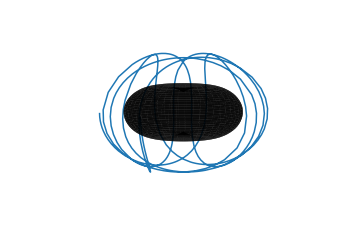
\includegraphics[width=0.8\linewidth]{img/3d-kerr-plot}
		\caption{A plot of a photon in the Kerr metric (r=3,$\theta=\frac{\pi}{2}$,$\varphi$=0,v=1,a=1,$\alpha$=0,$\delta$=-$\mbox{Arcsin}(\frac{1}{3})$}
	\end{minipage}%
	\begin{minipage}{0.5\textwidth}
		\centering
		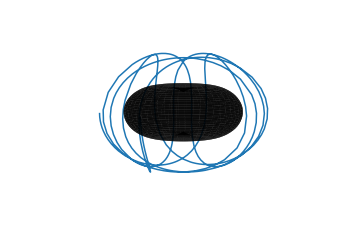
\includegraphics[width=0.8\linewidth]{img/3d-kerr-plot}
		\caption{A plot of a photon in the Kerr metric (r=3,$\theta=\frac{\pi}{2}$,$\varphi$=0,v=1,a=1,$\alpha$=0,$\delta$=-$\mbox{Arcsin}(\frac{1}{3})$}
	\end{minipage}
\end{figure}



\appendix
%\include{appendix1}
%\include{appendix2}

%\nocite{}
\bibliographystyle{plain}
\bibliography{bibliography}{}
\end{document}